\documentclass{article}[12pt]
\usepackage{verbatim}
\usepackage{graphicx}

\title{CS246 Assignment 1}
\author{Nissan Pow}

\begin{document}
\maketitle

\section*{Problem 1 - 7.2(a)}
\begin{enumerate}
  \item Sender - Create and send email(s).
  \item Recipient(s) - Retrieve email(s) from the server.
  \item System Administrator - Perform regular maintenance for the server (security updates, patches, etc).
\end{enumerate}

\section*{Problem 2 - 7.3(a)}
\begin{enumerate}
  \item Customer - Make reservation(s) and purchase ticket(s).
  \item Database - Maintains up-to-date information on flight schedules and pricing information, to be provided upon request.
\end{enumerate}

\section*{Problem 3 - 7.4(a)}
\begin{enumerate}
  \item Librarian - Performs the checkout of the item(s).
  \item Database - Maintains up-to-date information on the status of items in the library (on-shelf, in-transit, borrowed, etc).
  \item Book - Provides the catalogue number to the system in order to update the database.
\end{enumerate}

\section*{Problem 4}
  \subsection*{7.2(b)}
    \begin{enumerate}
      \item Compose an email - the user creates a draft of an email, which can be dispatched immediately or stored for future usage.
      \item Send email - the user dispatches the email to the recipient(s).
    \end{enumerate}

  \subsection*{7.3(b)}
    \begin{enumerate}
      \item Search for available flights - the user enters the flight information, and searches for all available matching flights. 
      \item Purchase ticket - after the user has found an acceptable flight, the user pays for the ticket.
    \end{enumerate}

  \subsection*{7.4(b)}
    \begin{enumerate}
      \item Return item(s) - the user returns item(s) that were previously checked out.
      \item Query outstanding item(s) - the librarian checks what item(s) that the user has outstanding.
    \end{enumerate}

  \subsection*{Use Case - Get Mail}
    \begin{enumerate}
      \item User logs in to email system.
      \item User queries email system for listing of new mail in the user's inbox.
      \item Email system forwards query to database.
      \item Database processes query and returns result of query to email system.
      \item System displays list of new mail in the user's inbox.
      \item User selects an email for viewing.
      \item System displays selected email. \\
            \emph{User repeats steps 2-7 until indicates done.}
      \item User logs out of email system.
    \end{enumerate} 

  \subsection*{Sequence diagram for getting mail.}
    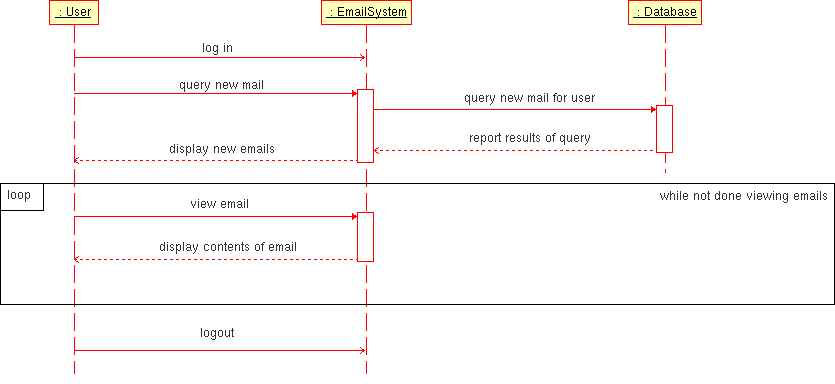
\includegraphics[scale=0.45]{get_mail.png}

  \subsection*{Use Case - Make a flight reservation.}
    \begin{enumerate}
      \item Customer logs in to online airline reservation system.
      \item Customer enters flight information.
      \item System queries database for flights matching entered criteria.
      \item Database returns result of query to system.
      \item System displays result of query to customer. \\
            \emph{Customer repeats steps 2-5 until indicates done.}
      \item Customer selects flight for reservation.
      \item System asks customer for appropriate payment.
      \item Customer pays appropriate fees and system handles payment.
      \item System logs reservation complete and sends payment information to database for updating.
      \item System displays confirmation of the reservation.
      \item Customer logs out of the online airline reservation system.
    \end{enumerate} 

  \subsection*{Sequence diagram for making a flight reservation.}
    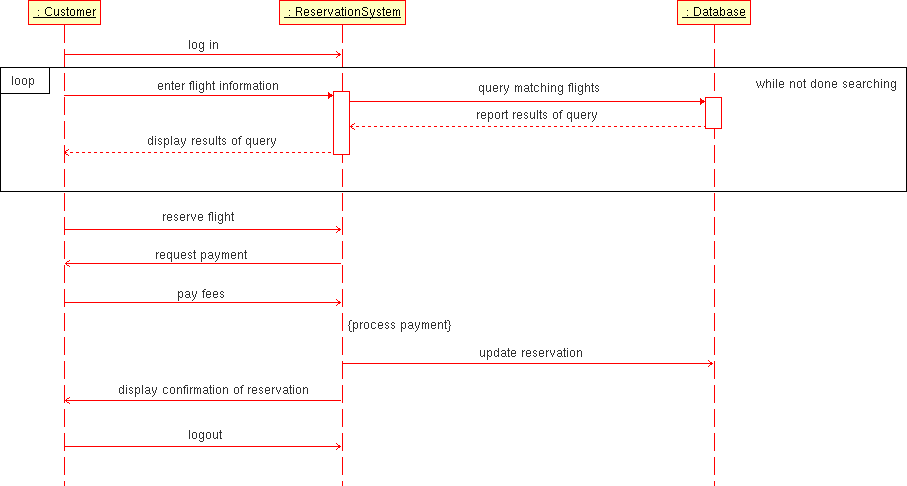
\includegraphics[scale=0.45]{make_reservation.png}

  \subsection*{Use Case - Borrow a library item.}
    \begin{enumerate}
      \item User arrives at item checkout location with item(s) to checkout.
      \item User presents library card to librarian.
      \item Librarian takes the library card and scans in the barcode.
      \item System displays user's account.
      \item Librarian scans the barcode of item.
      \item System sends checkout information to the database for updating. 
      \item System updates user's account with newly checked out item. \\
            \emph{Librarian repeats steps 5-9 until indicates done.}
      \item System terminates checkout and presents receipt.
      \item User leaves with receipt and item(s).
    \end{enumerate} 

  \subsection*{Sequence diagram for borrowing library items.}
    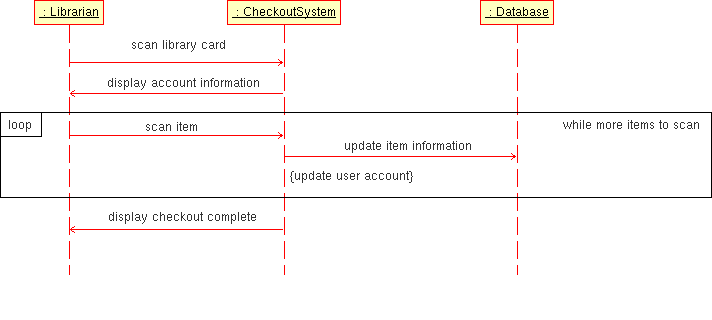
\includegraphics[scale=0.45]{checkout_item.png}

\section*{Problem 5}
  \subsection*{Use case diagram for an online airline reservation system.}
    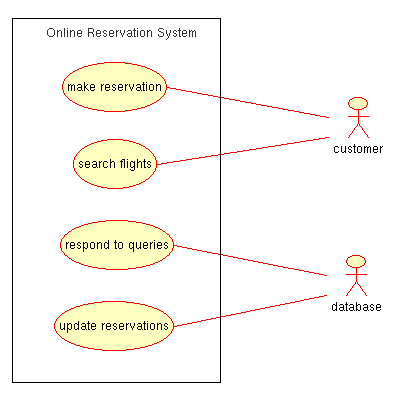
\includegraphics[scale=0.5]{make_reservation(ucd).png}

\section*{Problem 6}

\subsection*{6. (a)}
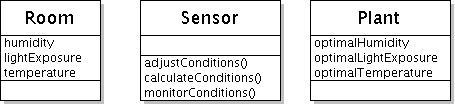
\includegraphics[scale=0.45]{a1q6a.png}


\subsection*{6. (b)}
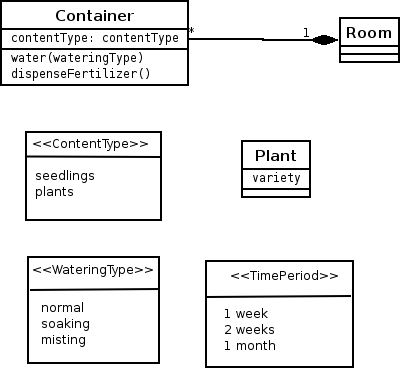
\includegraphics[scale=0.45]{a1q6b.png}


\subsection*{6. (c)}
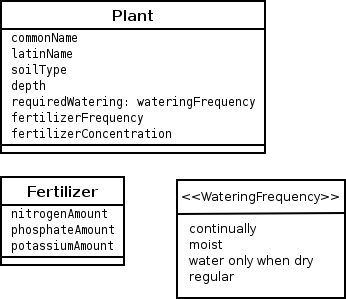
\includegraphics[scale=0.45]{a1q6c.png}

\end{document}

